% Paper 1 — LNCS (Springer) format, targeting ICDAR/ICFHR/DAS.
% Compile with XeLaTeX or LuaLaTeX for Devanagari examples (fontspec), or
% comment the fontspec block and the \dn{} examples to build with pdfLaTeX.
% Get llncs.cls from https://www.springer.com/gp/computer-science/lncs
\documentclass{llncs}

\usepackage{graphicx}
\usepackage{booktabs}
\usepackage{amsmath}
\usepackage{url}
% --- Devanagari support (XeLaTeX/LuaLaTeX) ---
\usepackage{iftex}
\ifPDFTeX
  \newcommand{\dn}[1]{\texttt{[Devanagari]}} % placeholder under pdfLaTeX
\else
  \usepackage{fontspec}
  \newfontfamily\devafont[Script=Devanagari,Path=./,
    UprightFont=NotoSansDevanagari-Regular.ttf]{NotoSansDevanagari}
  \newcommand{\dn}[1]{{\devafont #1}}
\fi

% Auto-generated result macros (run: python -m experiments.paper1.inject_numbers)
% Auto-generated by paper1/experiments/inject_numbers.py — do not edit.
% base_prep (n=12869)
\newcommand{\cerBasePrep}{0.1695}
\newcommand{\aerBasePrep}{0.2213}
\newcommand{\waccBasePrep}{0.6461}
\newcommand{\cerloBasePrep}{0.1643}
\newcommand{\cerhiBasePrep}{0.1745}
\newcommand{\paramsBasePrep}{184.08M}
% lora_r4_attn (n=12869)
\newcommand{\cerLoraFourAttn}{0.1141}
\newcommand{\aerLoraFourAttn}{0.1466}
\newcommand{\waccLoraFourAttn}{0.7534}
\newcommand{\cerloLoraFourAttn}{0.1099}
\newcommand{\cerhiLoraFourAttn}{0.1185}
\newcommand{\paramsLoraFourAttn}{0.59M}
% lora_r8_attn (n=12869)
\newcommand{\cerLoraEightAttn}{0.1095}
\newcommand{\aerLoraEightAttn}{0.1411}
\newcommand{\waccLoraEightAttn}{0.7614}
\newcommand{\cerloLoraEightAttn}{0.1053}
\newcommand{\cerhiLoraEightAttn}{0.1139}
\newcommand{\paramsLoraEightAttn}{1.18M}
% lora_r16_attn (n=12869)
\newcommand{\cerLoraSixteenAttn}{0.1065}
\newcommand{\aerLoraSixteenAttn}{0.1368}
\newcommand{\waccLoraSixteenAttn}{0.7691}
\newcommand{\cerloLoraSixteenAttn}{0.1022}
\newcommand{\cerhiLoraSixteenAttn}{0.1108}
\newcommand{\paramsLoraSixteenAttn}{2.36M}
% lora_r32_attn (n=12869)
\newcommand{\cerLoraThirtytwoAttn}{0.1030}
\newcommand{\aerLoraThirtytwoAttn}{0.1326}
\newcommand{\waccLoraThirtytwoAttn}{0.7760}
\newcommand{\cerloLoraThirtytwoAttn}{0.0988}
\newcommand{\cerhiLoraThirtytwoAttn}{0.1075}
\newcommand{\paramsLoraThirtytwoAttn}{4.72M}
% lora_r16_attn_ffn (n=12869)
\newcommand{\cerLoraSixteenAttnFfn}{0.1022}
\newcommand{\aerLoraSixteenAttnFfn}{0.1315}
\newcommand{\waccLoraSixteenAttnFfn}{0.7774}
\newcommand{\cerloLoraSixteenAttnFfn}{0.0981}
\newcommand{\cerhiLoraSixteenAttnFfn}{0.1062}
\newcommand{\paramsLoraSixteenAttnFfn}{4.62M}
% lora_r16_legacy (n=12869)
\newcommand{\cerLoraSixteenLegacy}{0.1013}
\newcommand{\aerLoraSixteenLegacy}{0.1307}
\newcommand{\waccLoraSixteenLegacy}{0.7786}
\newcommand{\cerloLoraSixteenLegacy}{0.0972}
\newcommand{\cerhiLoraSixteenLegacy}{0.1054}
\newcommand{\paramsLoraSixteenLegacy}{4.62M}
% full_ft (n=12869)
\newcommand{\cerFullFt}{0.0961}
\newcommand{\aerFullFt}{0.1192}
\newcommand{\waccFullFt}{0.7980}
\newcommand{\cerloFullFt}{0.0921}
\newcommand{\cerhiFullFt}{0.1005}
\newcommand{\paramsFullFt}{184.08M}
% lora_r16_attn_synth25: no results yet
\newcommand{\cerSynthTwoFive}{--}
\newcommand{\aerSynthTwoFive}{--}
\newcommand{\waccSynthTwoFive}{--}
\newcommand{\cerloSynthTwoFive}{--}
\newcommand{\cerhiSynthTwoFive}{--}
\newcommand{\paramsSynthTwoFive}{--}
% lora_r16_attn_synth50: no results yet
\newcommand{\cerSynthFive}{--}
\newcommand{\aerSynthFive}{--}
\newcommand{\waccSynthFive}{--}
\newcommand{\cerloSynthFive}{--}
\newcommand{\cerhiSynthFive}{--}
\newcommand{\paramsSynthFive}{--}
% lora_r16_attn_synth100: no results yet
\newcommand{\cerSynthTen}{--}
\newcommand{\aerSynthTen}{--}
\newcommand{\waccSynthTen}{--}
\newcommand{\cerloSynthTen}{--}
\newcommand{\cerhiSynthTen}{--}
\newcommand{\paramsSynthTen}{--}
% raw_pipeline_archive/base_checkpoint_m16 (n=12869)
\newcommand{\cerBaseRaw}{0.5297}
\newcommand{\aerBaseRaw}{0.6971}
\newcommand{\waccBaseRaw}{0.1192}
\newcommand{\cerloBaseRaw}{0.5250}
\newcommand{\cerhiBaseRaw}{0.5349}
\newcommand{\paramsBaseRaw}{184.08M}


\begin{document}

\title{Parameter-Efficient Adaptation of TrOCR for Devanagari Handwritten
Word Recognition}
\titlerunning{Parameter-Efficient TrOCR for Devanagari}

\author{Samir Wagle\inst{1} \and Manish~...\inst{1}}
\institute{Tribhuvan University, Kathmandu, Nepal\\
\email{samir@redtab.xyz}}

\maketitle

\begin{abstract}
Devanagari handwritten text recognition lags Latin-script systems, and the
transformer models that close this gap are costly to fine-tune for
low-resource settings. We present a systematic study of parameter-efficient
adaptation of TrOCR for Devanagari handwritten word recognition on the
IIIT-INDIC-HW-WORDS (Hindi) benchmark. We ablate LoRA rank and target-module
placement against full fine-tuning and zero-shot bounds, and show that
adapters training 2.5\% of model parameters recover 93\% of the full
fine-tuning improvement (CER \cerBasePrep{} $\rightarrow$
\cerLoraSixteenLegacy{} vs.\ \cerFullFt{}), with feed-forward placement
beating higher attention rank at a matched budget. We further identify input-distribution parity as a dominant
and previously unreported factor: fine-tuning on raw word strips while the
base checkpoint expects foreground-cropped, square-padded inputs
\emph{degrades} recognition below the unadapted baseline (CER
\cerBaseRaw{} $\rightarrow$ \cerLoraSixteenLegacy{} after alignment), an
effect invisible to training loss. Finally, we introduce akshara-level
evaluation for Devanagari: an orthographic-syllable error rate and an error
taxonomy separating conjunct, matra, and nasalization-sign failures, showing
that codepoint-level CER systematically misrepresents which linguistic units
fail. Code, adapters, and evaluation tooling are released.
\keywords{Handwritten text recognition \and Devanagari \and TrOCR \and
LoRA \and Parameter-efficient fine-tuning.}
\end{abstract}

\section{Introduction}

Handwritten text recognition (HTR) for Devanagari — the script of Hindi,
Nepali, Marathi, and Sanskrit, used by over 600 million people — remains
substantially behind Latin-script HTR. The script's properties make word
recognition harder than its Latin counterpart: consonants combine with
dependent vowel signs (\emph{matras}) above, below, before, and after the
base glyph; consonant clusters fuse into \emph{conjunct} ligatures
(e.g.\ \dn{क्ष}, \dn{त्र}) whose shapes are not compositional; and the
headline (\emph{shirorekha}) connects glyphs within a word, defeating
segmentation-based pipelines.

Transformer encoder–decoder models such as TrOCR~\cite{li2023trocr} transfer
well to new scripts, but full fine-tuning of a $\sim$190M-parameter model is
expensive in the low-resource settings where Indic HTR is most needed.
Low-rank adaptation (LoRA)~\cite{hu2022lora} promises the same adaptation at
a fraction of the trainable parameters, but no systematic study exists for
Devanagari: which layers to adapt, at what rank, and what the gap to full
fine-tuning is.

This paper contributes:
\begin{enumerate}
  \item \textbf{A systematic PEFT study for Devanagari word recognition.} We
  ablate LoRA rank ($r \in \{4, 8, 16, 32\}$) and target-module placement
  (attention-only vs.\ attention+FFN) on IIIT-INDIC-HW-WORDS
  Hindi~\cite{gongidi2021iiitindic}, against zero-shot and full fine-tuning
  bounds.
  \item \textbf{An input-parity finding.} Fine-tuning on raw word images
  while the base checkpoint was trained on foreground-cropped, square-padded
  inputs \emph{reduces} word accuracy from \waccBaseRaw{} to
  $\sim$0.02 despite converging training loss — the model visibly loses
  matra recognition. Restoring preprocessing parity flips the result. We
  argue input-distribution parity is a necessary control that PEFT studies
  on pretrained OCR models currently omit.
  \item \textbf{Akshara-level evaluation.} We propose evaluating Devanagari
  HTR at the orthographic-syllable (akshara) level, with an error taxonomy
  that separates conjunct substitutions, matra errors, and
  nasalization-sign errors. This reveals failure modes that codepoint CER
  conflates.
\end{enumerate}

\section{Related Work}

\paragraph{Transformer HTR and TrOCR.} TrOCR~\cite{li2023trocr} pairs a ViT
encoder with an autoregressive text decoder, pretrained on synthetic and
labeled text lines. It transfers to new scripts by replacing the tokenizer
and fine-tuning; community checkpoints exist for
Devanagari~\cite{paudelTrocrDevanagari}, and our study adapts one such
checkpoint rather than the English original, isolating the adaptation
question from the script-transfer question.

\paragraph{Parameter-efficient fine-tuning for OCR.}
DLoRA-TrOCR~\cite{chang2024dlora} applies weight-decomposed LoRA to TrOCR for
mixed handwritten/printed English text, establishing that PEFT is viable for
OCR transformers. Our work differs in three ways: we study an abugida whose
orthography stresses the decoder differently (matras, conjuncts); we ablate
\emph{where} adapters go, not only their rank; and we evaluate at the
akshara level. To our knowledge no PEFT study exists for any Indic script.

\paragraph{Indic HTR.} IIIT-INDIC-HW-WORDS~\cite{gongidi2021iiitindic}
established word-level benchmarks across ten Indic scripts with CRNN-style
baselines. Subsequent Devanagari work has largely used CNN/RNN hybrids;
transformer adaptation results on this benchmark are scarce, and none report
parameter-efficiency trade-offs.

\paragraph{Synthetic handwriting for augmentation.} Latent diffusion
generators such as WordStylist~\cite{nikolaidou2023wordstylist} and
DiffusionPen~\cite{nikolaidou2024diffusionpen} produce training data that
improves Latin-script HTR. No such generator exists for Devanagari; we
develop one, and the corresponding augmentation study, in a companion
paper.

\section{Method}

\subsection{Base Model and LoRA Placement}

We adapt \texttt{trocr-devanagari-2}~\cite{paudelTrocrDevanagari}, a
VisionEncoderDecoder checkpoint (ViT-base encoder, byte-level BPE decoder
tokenizer covering Devanagari) previously fine-tuned for Devanagari, totaling
184M parameters. LoRA adapters with scaling $\alpha = 2r$ and dropout $0.05$
are inserted into one of three module sets:
\begin{itemize}
  \item \textbf{attn}: encoder/decoder attention projections
  (query, key, value, output);
  \item \textbf{attn+ffn}: additionally the feed-forward projections;
  \item \textbf{legacy}: the suffix-matched set
  \{\texttt{query}, \texttt{key}, \texttt{value}, \texttt{dense}\} used by
  our originally deployed adapter, which via suffix matching also captures
  encoder FFN layers — included to quantify the effect of unintentional
  placement.
\end{itemize}
At $r{=}16$ these train \paramsLoraSixteenAttn{} (attn) to
\paramsLoraSixteenLegacy{} (legacy) parameters — under 3\% of the model.
Full fine-tuning (\paramsFullFt{}) provides the upper bound; the unadapted
checkpoint provides the lower.

\subsection{Input-Distribution Parity}
\label{sec:parity}

The base checkpoint was trained on word images that were foreground-cropped
and, for aspect ratios above 2.2, padded to a white square before ViT
resizing. The benchmark's raw images are wide strips (typical AR $> 3$).
Passing them directly to the ViT processor squashes them anisotropically —
a different input distribution from the checkpoint's.

We therefore train and evaluate under \emph{preprocessing parity}: the same
crop/pad transform as the checkpoint's original regime. Section~\ref{sec:results-parity}
quantifies what happens without it. We treat this as an experimental control,
not a trick: any PEFT study on a pretrained OCR model implicitly chooses an
input distribution, and the choice can dominate the effect being measured.

\subsection{Akshara-Level Evaluation}
\label{sec:akshara}

Codepoint-level CER treats the conjunct \dn{क्ष} (three codepoints) and the
simple consonant \dn{क} (one) asymmetrically, and scatters a single
perceptual error across multiple codepoint edits. We segment NFC-normalized
text into \emph{aksharas} — orthographic syllables of the form
$(C\,\text{virama})^{*}\,C\,(\text{nukta})?\,(\text{matra})?\,(\text{sign})^{*}$
— and report:
\begin{itemize}
  \item \textbf{AER}: Levenshtein distance over akshara sequences,
  normalized by reference length;
  \item \textbf{an error taxonomy} from the akshara-level alignment:
  \emph{conjunct substitution} (either side contains a virama-joined
  cluster), \emph{matra error} (same consonant skeleton, different vowel
  marking), \emph{nasalization-sign error} (anusvara/candrabindu/visarga
  only), \emph{base substitution}, and insertions/deletions.
\end{itemize}
All text is Unicode-NFC-normalized before scoring; without this, visually
identical predictions differing only in codepoint composition inflate CER.

\section{Experimental Setup}

\textbf{Data.} IIIT-INDIC-HW-WORDS Hindi~\cite{gongidi2021iiitindic,c3rl2024iiitindicHindi}:
$\sim$70k train / 12.9k validation / 12.9k test word images from the official
splits. No writer overlap handling is needed at word level.
\textbf{Training.} Seed 42; AdamW; LR $5{\times}10^{-5}$, batch 16, 2 epochs
(LoRA) / LR $2{\times}10^{-5}$, batch 8, 1 epoch (full FT);
beam search (4 beams) for generation; max generation length 32 tokens.
All runs fit a single NVIDIA T4 (Kaggle free tier) at $\sim$70--90 minutes
per LoRA configuration, making the study reproducible without datacenter
hardware.
\textbf{Metrics.} CER with 95\% percentile-bootstrap CIs (1{,}000
resamples), AER (Sect.~\ref{sec:akshara}), and word recognition accuracy,
all on the official test split.

\section{Results}

\subsection{Main Comparison and LoRA Ablation}

% Generated: experiments/paper1/results/tables/tables.tex (Table tab:main)
\begin{table}[t]
  \centering
  \caption{Test-split results on IIIT-INDIC-HW-WORDS-Hindi. CER: character error rate (NFC codepoints); AER: akshara error rate; WAcc: word recognition accuracy.}
  \label{tab:main}
  \begin{tabular}{lrrrr}
    \toprule
    Run & Trainable & CER $\downarrow$ & AER $\downarrow$ & WAcc $\uparrow$ \\
    \midrule
    full\_ft & 184.08M & 0.0961 & 0.1192 & 0.7980 \\
    lora\_r16\_legacy & 4.62M & 0.1013 & 0.1307 & 0.7786 \\
    lora\_r16\_attn\_ffn & 4.62M & 0.1022 & 0.1315 & 0.7774 \\
    lora\_r32\_attn & 4.72M & 0.1030 & 0.1326 & 0.7760 \\
    lora\_r16\_attn & 2.36M & 0.1065 & 0.1368 & 0.7691 \\
    lora\_r8\_attn & 1.18M & 0.1095 & 0.1411 & 0.7614 \\
    lora\_r4\_attn & 0.59M & 0.1141 & 0.1466 & 0.7534 \\
    base\_prep & 184.08M & 0.1695 & 0.2213 & 0.6461 \\
    \bottomrule
  \end{tabular}
\end{table}


Table~\ref{tab:main} reports the full matrix; Fig.~\ref{fig:rank} plots CER
against trainable parameters.

\begin{figure}[t]
\centering
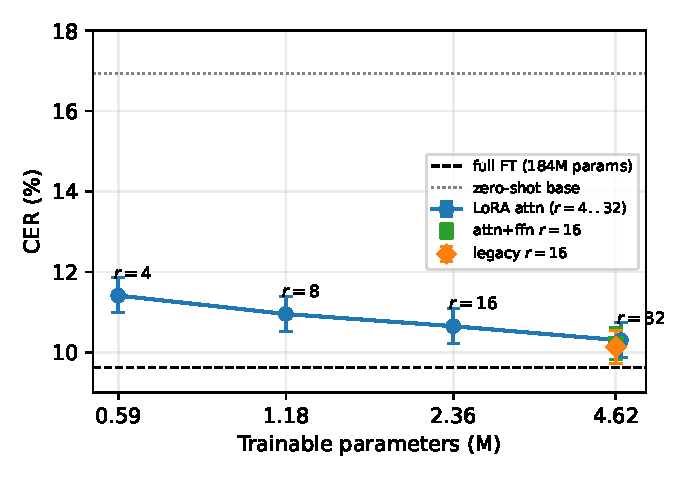
\includegraphics[width=0.82\linewidth]{figures/rank_curve.pdf}
\caption{Test CER (\%, 95\% bootstrap CIs) vs.\ trainable parameters.
The attention-only rank curve improves monotonically but sub-linearly in
$\log r$; at a matched $\sim$4.6M-parameter budget, spending capacity on FFN
modules (attn+ffn, legacy) outperforms doubling attention rank ($r{=}32$).}
\label{fig:rank}
\end{figure}

\textbf{Rank.} With attention-only placement, CER falls monotonically with
rank — \cerLoraFourAttn{} ($r{=}4$) $\rightarrow$ \cerLoraEightAttn{}
($r{=}8$) $\rightarrow$ \cerLoraSixteenAttn{} ($r{=}16$) $\rightarrow$
\cerLoraThirtytwoAttn{} ($r{=}32$) — but with diminishing returns: each rank
doubling buys roughly 0.4 CER points, then 0.3, then 0.35.
\textbf{Placement.} At a matched parameter budget ($\sim$4.6M), moving
capacity into feed-forward modules beats raising attention rank: attn+ffn at
$r{=}16$ (\cerLoraSixteenAttnFfn{}) and the legacy suffix-matched set
(\cerLoraSixteenLegacy{}) both outperform attention-only $r{=}32$
(\cerLoraThirtytwoAttn{}). \textbf{Gap to full fine-tuning.} The best
adapter (legacy, \paramsLoraSixteenLegacy{} trainable parameters — 2.5\% of
the model) reaches CER \cerLoraSixteenLegacy{} against \cerFullFt{} for full
fine-tuning of all \paramsFullFt{} parameters. A paired bootstrap over the
12{,}869 test words puts the difference at $+0.41$ CER points, 95\% CI
$[0.08, 0.76]$ ($p \approx 0.009$, 2{,}000 resamples): full fine-tuning is
statistically better, but the adapter recovers 93\% of the zero-shot
$\rightarrow$ full-FT improvement (CER \cerBasePrep{} $\rightarrow$
\cerFullFt{}) — and lifts word accuracy from \waccBasePrep{} to
\waccLoraSixteenLegacy{} — while training 40$\times$ fewer parameters.
\textbf{Seed robustness.} Repeating both headline configurations across
three seeds (42--44) gives CER $0.1020 \pm 0.0010$ (best adapter) and
$0.0953 \pm 0.0008$ (full FT; mean $\pm$ std): seed variance is an order
of magnitude smaller than every effect we report.

\subsection{The Cost of Ignoring Input Parity}
\label{sec:results-parity}

Under the raw-input regime, one epoch of LoRA fine-tuning converges in
training loss (6.25 $\rightarrow$ 0.34) yet \emph{collapses} generation:
word accuracy falls from \waccBaseRaw{} (unadapted, raw inputs) to 0.022,
with predictions retaining consonant skeletons but dropping matras
(\dn{अनाथों} $\rightarrow$ \dn{अनथथय}). With preprocessing parity restored,
the same 400-sample smoke configuration reaches CER 0.178 — and the
unadapted baseline itself improves from \cerBaseRaw{} to \cerBasePrep{}.
Training loss is computed under teacher forcing and cannot reveal this
failure; only generation-based evaluation does. We recommend PEFT studies on
pretrained OCR models report their input pipeline as part of the method.

\subsection{Akshara-Level Error Analysis}

\begin{table}[t]
\centering
\caption{Akshara-level error taxonomy on the test set (42{,}374 reference
aksharas), for full fine-tuning and the best adapter.}
\label{tab:taxonomy}
\begin{tabular}{lrrrr}
\toprule
& \multicolumn{2}{c}{full FT} & \multicolumn{2}{c}{LoRA legacy $r{=}16$} \\
Error category & Count & \% & Count & \% \\
\midrule
Base consonant substitution & 2015 & 39.1 & 2220 & 40.1 \\
Conjunct substitution       & 1608 & 31.2 & 1580 & 28.6 \\
Deletion                    &  530 & 10.3 &  583 & 10.5 \\
Matra (dependent vowel)     &  512 &  9.9 &  586 & 10.6 \\
Insertion                   &  230 &  4.5 &  280 &  5.1 \\
Nasalization/visarga sign   &  174 &  3.4 &  197 &  3.6 \\
Conjunct insertion/deletion &   83 &  1.6 &   85 &  1.5 \\
\midrule
Total akshara edits         & 5152 & & 5531 & \\
\bottomrule
\end{tabular}
\end{table}

Table~\ref{tab:taxonomy} breaks the akshara-level alignment into
script-aware categories. Two findings stand out. First, \textbf{conjuncts
are the hard case}: aksharas containing virama-joined clusters err at rate
0.170 (full FT) and 0.190 (LoRA) against 0.108 and 0.115 for simple
aksharas — roughly $1.6\times$ — and words with $2{+}$ conjuncts carry
nearly twice the akshara error rate of conjunct-free words (0.20 vs.\ 0.11).
Second, \textbf{script-specific categories account for $\sim$45\% of all
errors}: conjunct substitutions ($\sim$30\%), matra errors ($\sim$10\%), and
nasalization-sign errors ($\sim$3.5\%) have no Latin-script analogue and are
invisible to plain CER, which scatters a single conjunct confusion across up
to three codepoint edits. The taxonomy also shows \emph{where} the extra
capacity of full fine-tuning goes: relative to LoRA it removes matra errors
($-13$\%) and base substitutions ($-9$\%), while conjunct substitutions are
essentially unchanged ($+2$\%), suggesting the residual conjunct difficulty
is a visual-encoder limitation that neither adapter capacity nor full
fine-tuning closes. Fig.~\ref{fig:qual} shows
representative cases.

\begin{figure}[t]
\centering
\setlength{\tabcolsep}{5pt}
\begin{tabular}{cll}
\toprule
Image & Reference & Predictions (full FT / LoRA) \\
\midrule
\raisebox{-0.4\height}{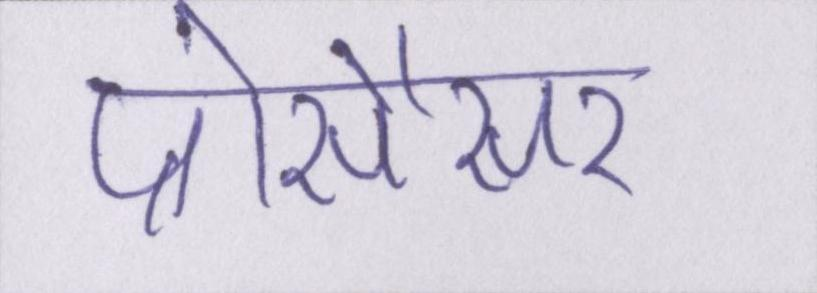
\includegraphics[height=18pt]{figures/qual_00019.png}} &
\dn{प्रोसैसर} & both correct \\
\raisebox{-0.4\height}{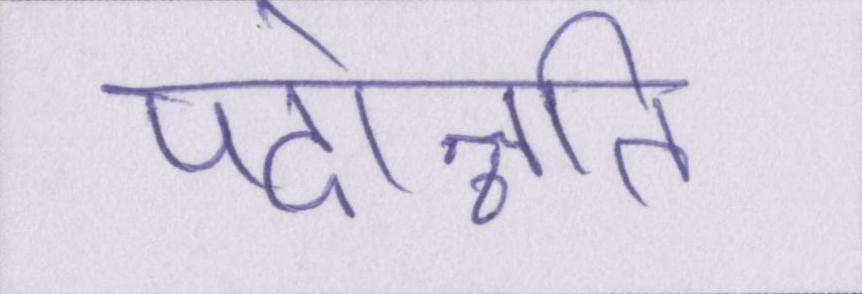
\includegraphics[height=18pt]{figures/qual_00084.png}} &
\dn{पदोन्नति} & both correct \\
\raisebox{-0.4\height}{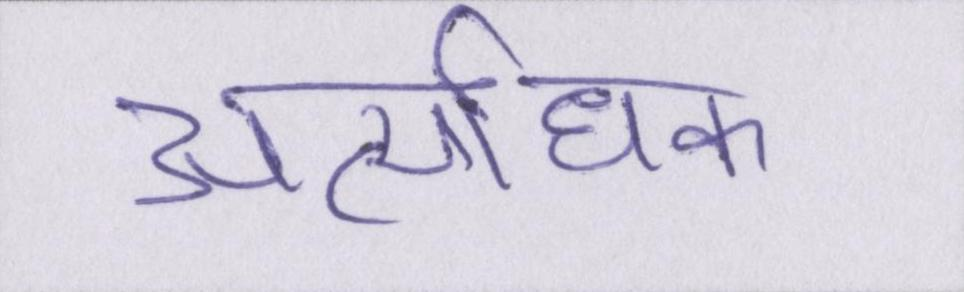
\includegraphics[height=18pt]{figures/qual_00063.png}} &
\dn{अत्यधिक} & \dn{अर्थशक} / \dn{अर्थशक} (conjunct) \\
\raisebox{-0.4\height}{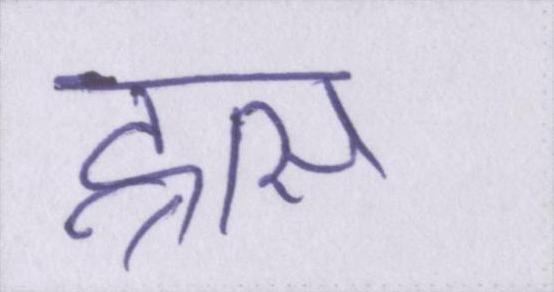
\includegraphics[height=18pt]{figures/qual_00026.png}} &
\dn{ह्रास} & \dn{द्वास} / \dn{द्वास} (conjunct) \\
\raisebox{-0.4\height}{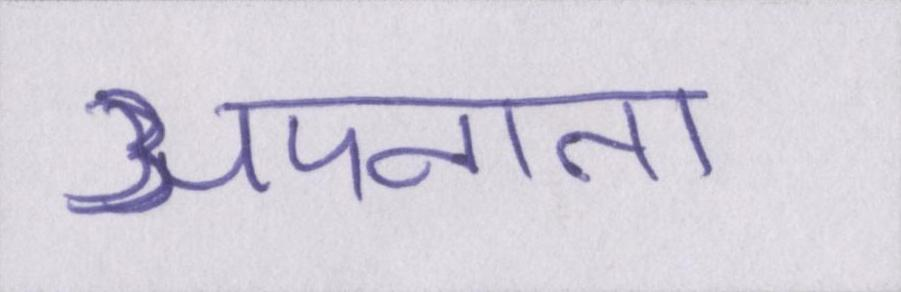
\includegraphics[height=18pt]{figures/qual_00138.png}} &
\dn{अपनाता} & \dn{अपनाना} / \dn{अपनाना} (base subst.) \\
\raisebox{-0.4\height}{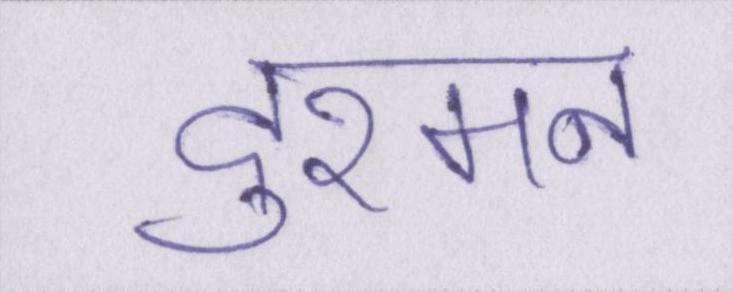
\includegraphics[height=18pt]{figures/qual_00296.png}} &
\dn{दुश्मन} & \dn{दुश्मन} / \dn{दुःशम} (LoRA only) \\
\bottomrule
\end{tabular}
\caption{Qualitative examples. Conjunct-dense words (\dn{प्रोसैसर},
\dn{पदोन्नति}) are often recognized exactly, but cursive or ambiguous
conjuncts (\dn{त्य}, \dn{ह्र}) trigger substitutions that both models share;
the last row shows a failure unique to the adapter.}
\label{fig:qual}
\end{figure}

\section{Conclusion}

We presented the first systematic parameter-efficient fine-tuning study for
Devanagari handwritten word recognition, an input-parity control that any
adaptation study on pretrained OCR checkpoints should adopt, and
akshara-level metrics that expose script-specific failure modes invisible
to codepoint CER. Adapters training 2.5\% of parameters recover 93\% of the
full fine-tuning gain, making high-quality Devanagari HTR trainable on
free-tier hardware. The error taxonomy identifies conjunct recognition as
the open problem: its error rate is $1.6\times$ that of simple aksharas and
is not reduced by full fine-tuning, motivating targeted synthetic data — the
subject of our companion work on Devanagari handwriting generation. Code, adapters, and the evaluation toolkit are available
at \url{https://github.com/USER/DevGen}.

\bibliographystyle{splncs04}
\bibliography{references}

\end{document}
